% Section 2 - Services
% Roberto Masocco <roberto.masocco@uniroma2.it>
% May 24, 2023

% ### Services ###
\section{Services}
\graphicspath{{figs/section2/}}

% --- ROS 2 services ---
\begin{frame}{ROS 2 services}{Basic client-server paradigm}
  ROS 2 extends the basic DDS messages adding two more \textbg{communication paradigms}: the first is the \textbg{service}. It allows nodes to establish quick and simple \textbg{client-server} communications.
  \begin{figure}
    \centering
    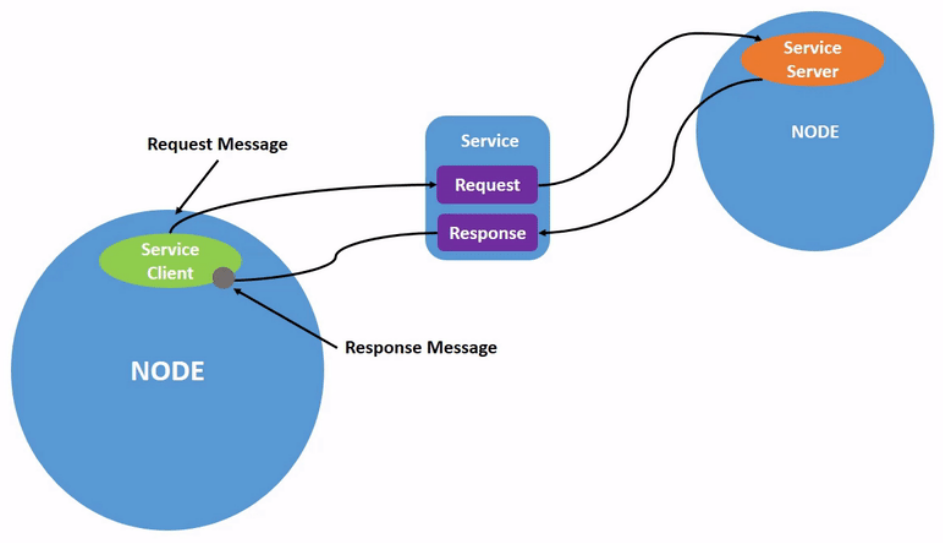
\includegraphics[scale=.33]{ros2Srv.png}
    \caption{Two nodes acting as service \emph{client} and \emph{server}.}
    \label{fig:ros2srv}
  \end{figure}
\end{frame}
\begin{frame}{ROS 2 services}{Communication overview}
  In actual ROS 2 applications:
  \begin{enumerate}
    \item The \textbg{client} sends a \textbg{request message} to the server.
    \item The \textbg{server} receives the request and processes it.
    \item Meanwhile, the \textbg{client} can either \textbg{block} waiting for the response or \textbg{synchronously poll} it.
    \item When done, the \textbg{server} sends a \textbg{response message} to the client.
    \item If waiting, the \textbg{client} awakes when receiving the reponse.
  \end{enumerate}
\end{frame}
\begin{frame}{ROS 2 services}{Coding hints for servers and clients}
  \begin{block}{Servers}
    Similarly to topic subscriptions, requests are processed in appropriate \textbf{callbacks}, taking \textbf{two arguments}, in which responses are also populated. The server object is as well only needed to instantiate the service.
  \end{block}
  \begin{block}{Clients}
    As per the previous dynamics, one has to \textbf{code each step} of the client side into their application using appropriate \textbf{ROS 2 APIs}. \textbf{The client object is used to send requests}, while \textbf{responses are handled as \texttt{future} objects\footnote{\href{https://en.cppreference.com/w/cpp/thread/future}{\color{blue}\underline{\texttt{std::future} - C++ Reference}}}}.
  \end{block}
\end{frame}

% --- Interface files - Services ---
\begin{frame}[fragile]{Interface files}{Services}
  The entire system is built on messages, so \textbg{combine two of them} in a single interface file, separated by \texttt{-{}-{}-}.\\
  Service file names end with \texttt{.srv}.
  \begin{columns}
  \column{.9\textwidth}
  % Listing: example_interfaces/srv/AddTwoInts service definition
  \begin{lstlisting}[language=ros2msg, caption=Definition of the \texttt{example\_interfaces/srv/AddTwoInts} service.]
# REQUEST
int64 a
int64 b
---
# RESPONSE
int64 sum\end{lstlisting}
  \end{columns}
\end{frame}

% --- Example - Simple service ---
\begin{frame}{Example}{Simple service}
  \begin{block}{}
    \centering
    Now go have a look at the \href{https://github.com/IntelligentSystemsLabUTV/ros2-examples/tree/humble/src/cpp/simple_service_cpp}{\color{blue}\underline{\texttt{ros2-examples/src/cpp/simple\_service\_cpp}}} package!
  \end{block}
\end{frame}
